% ==============================================================================
% EE413A
% Lab 2
% The Operational Amplifier.
%
% Author:
% Jonas Sjöberg     <tel12jsg@student.hig.se>
% Esther Hedlund    <tfk13ehd@student.hig.se>
% 
% TODO: License.
% ==============================================================================


% ==============================================================================
% INCLUDES AND CONFIGURATION
% ==============================================================================

\documentclass[]{article}

\usepackage[utf8]{inputenc}
\usepackage{siunitx} % Provides the \SI{}{} and \si{} command for typesetting SI
\usepackage{amssymb,amsmath}
\usepackage{graphicx}
\usepackage{longtable,booktabs}
\IfFileExists{microtype.sty}{\usepackage{microtype}}{}

\setlength\parindent{0pt} % Removes all indentation from paragraphs




% ==============================================================================
% DOCUMENT METADATA 
% ==============================================================================

\title{EE413 \\ Lab 005 \\ the Operational Amplifier}
\author{{Jonas Sjöberg} \and {Esther Hedlund}}

\date{}

\begin{document}

\maketitle

\begin{center}
\begin{tabular}{l r}
Data Performed: & 26 November 2014 \\
Instructor: TODO
\end{tabular}
\end{center}

% ==============================================================================
% ABSTRACT
% ==============================================================================
\begin{abstract}
"This lab is meant to teach and show the practical use of NPN bjt amplifiers.
The lab includes constructing and measuring DC circuits, calculating biasing networks,
amplification, bandwidth and plotting characteristic curves of circuit parameters."
\end{abstract}

%{
%\hypersetup{linkcolor=black}
%\setcounter{tocdepth}{3}
%\tableofcontents
%}

\newpage

\section{Inverting DC Amplifier}\label{inverting-dc-amplifier}

\subsection{Theory}\label{theory}

\begin{figure}[htbp]
    \centering
        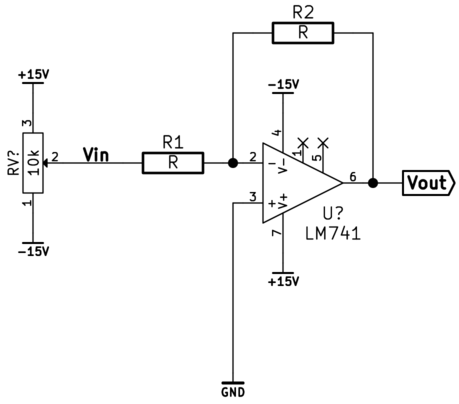
\includegraphics{img/invDCamp.png}
    \caption{Inverting DC amplifier}
    \label{fig:invDCamp}
\end{figure}

The basic topology for an inverting amplifier is shown in ~\ref{fig:invDCamp}.
Gain, Av, can be expressed as a ratio of the feedback impedance to the
input impedance. A fraction of the output is fed back, causing the op
amp to compensate and in effect amplify.

\begin{equation}
A_v = \frac{R_2}{R_1}
\end{equation}

The circuit gain for ideal components is therefore;

For $R_2 = 100k\Omega$:

\begin{align} 
A_v     &= \frac{V_{out}}{V_{in}} = -\frac{R_2}{R_1}\\
        &= \frac{100k\Omega}{10k\Omega} = 10\\
        &= 20 \times \log{\frac{10}{1}} = 20dB  
\end{align}

For $R_2 = 10k\Omega$:

\begin{align} 
A_v     &= \frac{V_{out}}{V_{in}} = -\frac{R_2}{R_1}\\
        &= \frac{10k\Omega}{10k\Omega} = 10\\
        &= 20 \times \log{\frac{1}{1}} = 0dB  
\end{align}

In both cases, the signal phase is inverted $180^\circ$.

\subsection{Measurements}\label{measurements}
\begin{table}[h]
  \centering
  \begin{tabular}{@{}lllll@{}}
    \toprule
    Uin (V) & Uout (V) & Av (x) &  &  \\ \midrule
    -0.105 & +1.087  & -10.54     &  &  \\
    -1.008  & +10.236   & -10.15     &  &  \\
    +1.004  & -10.104   & -10.06     &  &  \\ \bottomrule
  \end{tabular}
  \caption{R2 = 100k$\Omega$}
  \label{invDCtable1}
\end{table}

\begin{table}[h]
  \centering
  \begin{tabular}{@{}lllll@{}}
    \toprule
    Uin (V) & Uout (V) & Av (x) &  &  \\ \midrule
    -0.1051 & +0.1051  & -1     &  &  \\
    -1.008  & +1.008   & -1     &  &  \\
    +1.004  & -1.004   & -1     &  &  \\ \bottomrule
  \end{tabular}
  \caption{R2 = 10k$\Omega$}
  \label{invDCtable2}
\end{table}


\section{Inverting AC Amplifier}\label{inverting-ac-amplifier}

\subsection{Oscilloscope shots}\label{oscilloscope-shots}

\subsection{Measurements}\label{measurements-1}

Measured amplification = --- Measured phase = 180 Theoretical amplifier
=\\Theoretical phase =

\begin{figure}[htbp]
\centering
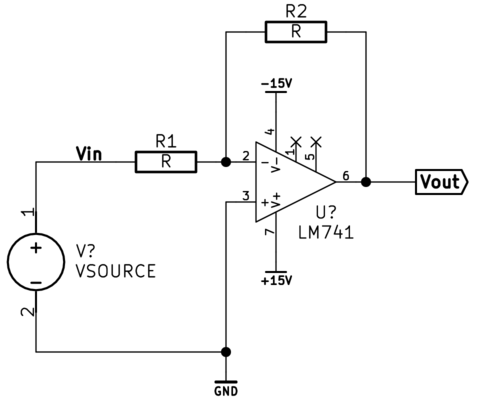
\includegraphics{img/invACamp.png}
\caption{Inverting AC amplifier}
\end{figure}

\section{Non-inverting DC Amplifier}\label{non-inverting-dc-amplifier}

Av = 1 + R2/R1

\subsection{Measurements}\label{measurements-2}

\begin{longtable}[c]{@{}lll@{}}
\toprule\addlinespace
Uin (V) & Uout (V) & Av (ggr)
\\\addlinespace
\midrule\endhead
+0.1007 & +0.2164 2 & .15
\\\addlinespace
+1.002 & +2.048 2 & .04
\\\addlinespace
-1.005 & -2.03 2 & .019
\\\addlinespace
\bottomrule
\addlinespace
\caption{R2 = 10k$\Omega$}
\end{longtable}

\begin{longtable}[c]{@{}lll@{}}
\toprule\addlinespace
Uin (V) & Uout (V) & Av (ggr)
\\\addlinespace
\midrule\endhead
+0.1009 & +1.178 & 11.67
\\\addlinespace
+1.1013 & +11.3 & 11.15
\\\addlinespace
-1.004 & -11.09 & 11.05
\\\addlinespace
\bottomrule
\addlinespace
\caption{R2 = 100k$\Omega$}
\end{longtable}

\begin{figure}[htbp]
\centering
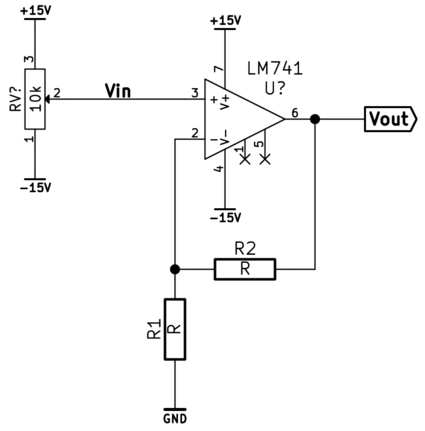
\includegraphics{img/noninvDCamp.png}
\caption{Non-inverting DC amplifier}
\end{figure}

\section{Non-inverting AC Amplifier}\label{non-inverting-ac-amplifier}

\subsection{Measurements}\label{measurements-3}

Input signal amplitude =\\Output signal amplitude =\\Measured
amplification =\\Measured phase =

Theoretical amplification = Theoretical phase =

\begin{figure}[htbp]
\centering
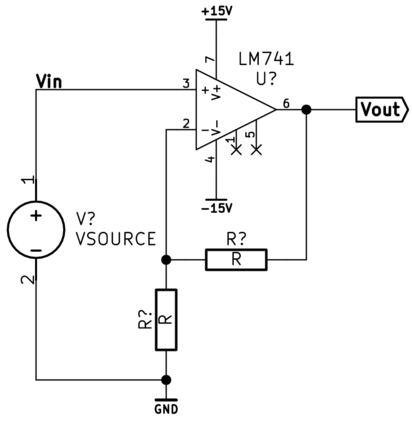
\includegraphics{img/noninvACamp.png}
\caption{Non-inverting AC amplifier}
\end{figure}

\section{Active full wave rectifier}\label{active-full-wave-rectifier}

Active rectifier does not suffer from the ``deadzone'' when the signal
is too small to turn on the rectifying diode. The op amp compensates for
the diode forward voltage drop. The circuit output is a full wave
rectified version of the signal, with a frequency limit mostly set by
the op amp bandwidth. Diode D2 prevents the op amp from hitting the rail
hard when D1 is reverse biased. This makes the recovery and rise time
faster when D1 biases on. This improves circuit response times.

\begin{figure}[htbp]
\centering
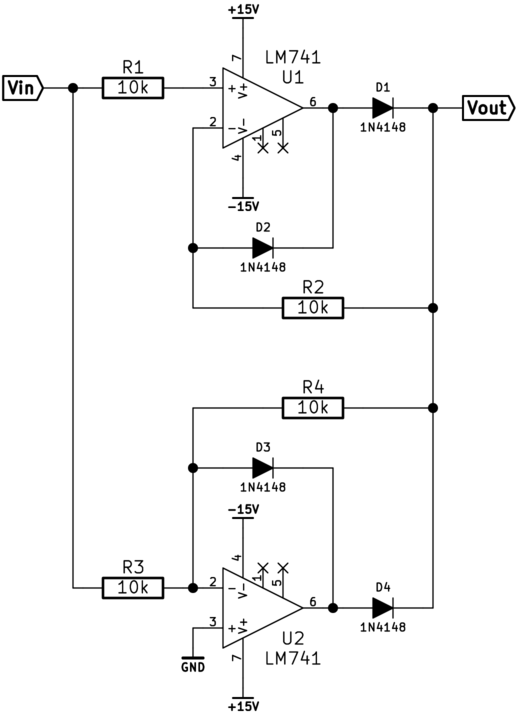
\includegraphics{img/fwr.png}
\caption{Active full wave rectifier}
\end{figure}

\end{document}
